\documentclass[11pt]{article}
\usepackage[margin=1in]{geometry}
\usepackage{amsmath,amssymb}
\usepackage{tikz}
\usepackage{pgfplots}
\usepackage{booktabs}
\usepackage{xcolor}

% Brand colors
\definecolor{garnet}{HTML}{73000A}
\definecolor{atlantic}{HTML}{466A9F}
\definecolor{congaree}{HTML}{1F414D}
\definecolor{horseshoe}{HTML}{65780B}
\definecolor{rose}{HTML}{CC2E40}
\definecolor{black90}{HTML}{363636}
\definecolor{black70}{HTML}{5C5C5C}
\definecolor{honeycomb}{HTML}{A49137}

\pgfplotsset{compat=1.18}

% Unit commands
\newcommand{\degC}{$^\circ$C}
\newcommand{\unit}[1]{\,\mathrm{#1}}

\title{\textbf{Heat Loss from Cylinder in Square Enclosure}}
\author{J.C. Vaught}
\date{\today}

\begin{document}
\maketitle

\section{Problem Statement}

Estimate the heat loss from an infinite steel cylinder enclosed in a square plywood box:
\begin{itemize}
    \item Cylinder diameter: $D = 25\unit{cm} = 0.25\unit{m}$
    \item Cylinder temperature: $T_{cyl} = 90$\degC
    \item Minimum gap between cylinder and box: $\delta = 10\unit{cm} = 0.10\unit{m}$
    \item Plywood thickness: $t = 1\unit{cm} = 0.01\unit{m}$
    \item Ambient temperature: $T_\infty = 20$\degC
    \item Air inside enclosure is stagnant (enclosed)
    \item Calculate heat loss per $L = 30\unit{cm}$ of length
\end{itemize}

\section{Geometry}

\begin{figure}[h]
\centering
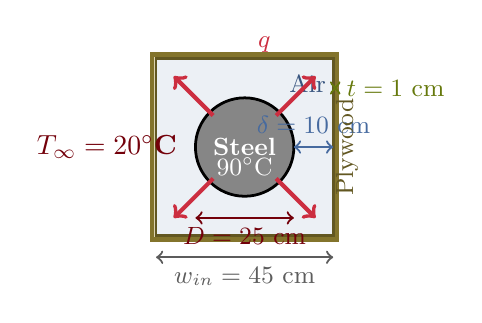
\begin{tikzpicture}[scale=5]
    % Outer plywood box
    \fill[honeycomb!40] (-0.235,-0.235) rectangle (0.235,0.235);
    \fill[white] (-0.225,-0.225) rectangle (0.225,0.225);

    % Inner air space
    \fill[atlantic!10] (-0.225,-0.225) rectangle (0.225,0.225);

    % Steel cylinder
    \fill[black90!60] (0,0) circle (0.125);
    \draw[line width=1pt] (0,0) circle (0.125);

    % Draw plywood outline
    \draw[line width=1.5pt, honeycomb!80!black] (-0.235,-0.235) rectangle (0.235,0.235);
    \draw[line width=1pt, honeycomb!60!black] (-0.225,-0.225) rectangle (0.225,0.225);

    % Dimension: cylinder diameter
    \draw[<->, line width=0.8pt, garnet] (-0.125,-0.18) -- (0.125,-0.18);
    \node[below, garnet, font=\small] at (0,-0.18) {$D = 25$ cm};

    % Dimension: gap
    \draw[<->, line width=0.8pt, atlantic] (0.125,0) -- (0.225,0);
    \node[above, atlantic, font=\small] at (0.175,0.01) {$\delta = 10$ cm};

    % Dimension: plywood thickness
    \draw[<->, line width=0.8pt, horseshoe] (0.225,0.15) -- (0.235,0.15);
    \node[right, horseshoe, font=\small] at (0.235,0.15) {$t = 1$ cm};

    % Dimension: inner box
    \draw[<->, line width=0.8pt, black70] (-0.225,-0.28) -- (0.225,-0.28);
    \node[below, black70, font=\small] at (0,-0.28) {$w_{in} = 45$ cm};

    % Labels
    \node[white, font=\bfseries\small] at (0,0) {Steel};
    \node[white, font=\small] at (0,-0.05) {90\degC};

    \node[atlantic!80!black, font=\small] at (0.16,0.16) {Air};

    \node[honeycomb!60!black, font=\small, rotate=90] at (0.26,0) {Plywood};

    % Temperature labels
    \node[garnet, font=\bfseries] at (-0.35,0) {$T_\infty = 20$\degC};

    % Heat flow arrows
    \draw[->, line width=1.5pt, rose] (0.08,0.08) -- (0.18,0.18);
    \draw[->, line width=1.5pt, rose] (-0.08,0.08) -- (-0.18,0.18);
    \draw[->, line width=1.5pt, rose] (0.08,-0.08) -- (0.18,-0.18);
    \draw[->, line width=1.5pt, rose] (-0.08,-0.08) -- (-0.18,-0.18);
    \node[rose, font=\small\bfseries] at (0.05,0.26) {$q$};
\end{tikzpicture}
\caption{Cross-section of steel cylinder inside square plywood enclosure.}
\label{fig:geometry}
\end{figure}

\subsection{Calculated Dimensions}

\begin{align}
    \text{Cylinder radius:} \quad r_i &= D/2 = 0.125\unit{m} \\
    \text{Inner box half-width:} \quad a_{in} &= r_i + \delta = 0.125 + 0.10 = 0.225\unit{m} \\
    \text{Inner box side:} \quad w_{in} &= 2 \times a_{in} = 0.45\unit{m} \\
    \text{Outer box side:} \quad w_{out} &= w_{in} + 2t = 0.47\unit{m}
\end{align}

\section{Thermal Resistance Network}

Heat flows through three resistances in series:

\begin{figure}[h]
\centering
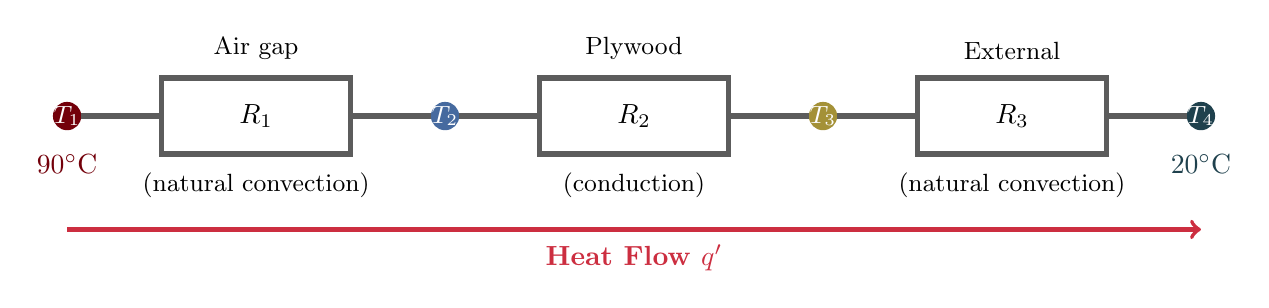
\begin{tikzpicture}[scale=1.2]
    % Nodes
    \fill[garnet] (0,0) circle (0.15);
    \node[white, font=\small\bfseries] at (0,0) {$T_1$};
    \node[below, garnet] at (0,-0.3) {90\degC};

    \fill[atlantic] (4,0) circle (0.15);
    \node[white, font=\small\bfseries] at (4,0) {$T_2$};

    \fill[honeycomb] (8,0) circle (0.15);
    \node[white, font=\small\bfseries] at (8,0) {$T_3$};

    \fill[congaree] (12,0) circle (0.15);
    \node[white, font=\small\bfseries] at (12,0) {$T_4$};
    \node[below, congaree] at (12,-0.3) {20\degC};

    % Resistances
    \draw[line width=2pt, black70] (0.15,0) -- (1,0);
    \draw[line width=2pt, black70] (1,-0.4) rectangle (3,0.4);
    \node[font=\bfseries] at (2,0) {$R_1$};
    \draw[line width=2pt, black70] (3,0) -- (3.85,0);

    \draw[line width=2pt, black70] (4.15,0) -- (5,0);
    \draw[line width=2pt, black70] (5,-0.4) rectangle (7,0.4);
    \node[font=\bfseries] at (6,0) {$R_2$};
    \draw[line width=2pt, black70] (7,0) -- (7.85,0);

    \draw[line width=2pt, black70] (8.15,0) -- (9,0);
    \draw[line width=2pt, black70] (9,-0.4) rectangle (11,0.4);
    \node[font=\bfseries] at (10,0) {$R_3$};
    \draw[line width=2pt, black70] (11,0) -- (11.85,0);

    % Labels
    \node[above, font=\small] at (2,0.5) {Air gap};
    \node[below, font=\small] at (2,-0.5) {(natural convection)};

    \node[above, font=\small] at (6,0.5) {Plywood};
    \node[below, font=\small] at (6,-0.5) {(conduction)};

    \node[above, font=\small] at (10,0.5) {External};
    \node[below, font=\small] at (10,-0.5) {(natural convection)};

    % Heat flow
    \draw[->, line width=1.5pt, rose] (0,-1.2) -- (12,-1.2);
    \node[rose, font=\bfseries] at (6,-1.5) {Heat Flow $q'$};
\end{tikzpicture}
\caption{Thermal resistance network (per unit length).}
\label{fig:resistance}
\end{figure}

\section{Material Properties}

\subsection{Air at Film Temperature}

Estimated film temperature in enclosure: $T_f \approx 55$\degC{} $= 328\unit{K}$

\begin{table}[h]
\centering
\caption{Air properties at $T_f = 55$\degC}
\begin{tabular}{lll}
\toprule
\textbf{Property} & \textbf{Symbol} & \textbf{Value} \\
\midrule
Thermal conductivity & $k_{air}$ & $0.0283\unit{W/(m \cdot K)}$ \\
Kinematic viscosity & $\nu$ & $1.82 \times 10^{-5}\unit{m^2/s}$ \\
Thermal diffusivity & $\alpha$ & $2.59 \times 10^{-5}\unit{m^2/s}$ \\
Thermal expansion coeff. & $\beta$ & $3.05 \times 10^{-3}\unit{K^{-1}}$ \\
Prandtl number & $Pr$ & 0.703 \\
\bottomrule
\end{tabular}
\end{table}

\subsection{Plywood}
\begin{equation}
    k_{plywood} \approx 0.12\unit{W/(m \cdot K)}
\end{equation}

\section{Resistance Calculations (Per Unit Length)}

\subsection{$R_1$: Enclosed Air Gap (Cylinder to Inner Plywood Surface)}

For a cylinder inside a square enclosure, the \textbf{shape factor} per unit length is:
\begin{equation}
    S = \frac{2\pi}{\ln(1.08 \times w_{in}/D)} = \frac{2\pi}{\ln(1.08 \times 0.45/0.25)} = \frac{2\pi}{\ln(1.944)} = \frac{2\pi}{0.665} = 9.45\unit{m^{-1}}
\end{equation}

For natural convection in the enclosure, we calculate the Rayleigh number using the minimum gap:
\begin{equation}
    Ra_\delta = \frac{g\beta\Delta T \delta^3}{\nu\alpha}
\end{equation}

Estimating $\Delta T \approx 57\unit{K}$ (between cylinder and inner plywood):
\begin{equation}
    Ra_\delta = \frac{9.81 \times 3.05 \times 10^{-3} \times 57 \times (0.10)^3}{1.82 \times 10^{-5} \times 2.59 \times 10^{-5}} = \boxed{3.62 \times 10^6}
\end{equation}

For enclosed spaces with $Ra > 10^4$, the Nusselt number correlation:
\begin{equation}
    Nu = 0.046 \times Ra_\delta^{1/3} = 0.046 \times (3.62 \times 10^6)^{1/3} = 0.046 \times 153 = \boxed{7.0}
\end{equation}

Effective thermal conductivity:
\begin{equation}
    k_{eff} = k_{air} \times Nu = 0.0283 \times 7.0 = 0.198\unit{W/(m \cdot K)}
\end{equation}

Thermal resistance of air gap:
\begin{equation}
    R_1 = \frac{1}{S \times k_{eff}} = \frac{1}{9.45 \times 0.198} = \boxed{0.534\unit{(m \cdot K)/W}}
\end{equation}

\subsection{$R_2$: Plywood Conduction}

For conduction through the plywood wall (approximated as a thin shell):
\begin{equation}
    P_{in} = 4 \times w_{in} = 4 \times 0.45 = 1.80\unit{m}
\end{equation}

\begin{equation}
    R_2 = \frac{t}{k_{plywood} \times P_{in}} = \frac{0.01}{0.12 \times 1.80} = \boxed{0.046\unit{(m \cdot K)/W}}
\end{equation}

\subsection{$R_3$: External Natural Convection}

For natural convection from the outer plywood surface to ambient air:
\begin{equation}
    P_{out} = 4 \times w_{out} = 4 \times 0.47 = 1.88\unit{m}
\end{equation}

Estimated heat transfer coefficient for natural convection from vertical surfaces:
\begin{equation}
    h_{ext} \approx 7\unit{W/(m^2 \cdot K)}
\end{equation}

\begin{equation}
    R_3 = \frac{1}{h_{ext} \times P_{out}} = \frac{1}{7 \times 1.88} = \boxed{0.076\unit{(m \cdot K)/W}}
\end{equation}

\section{Total Heat Loss Calculation}

\subsection{Total Thermal Resistance}
\begin{equation}
    R_{total} = R_1 + R_2 + R_3 = 0.534 + 0.046 + 0.076 = \boxed{0.656\unit{(m \cdot K)/W}}
\end{equation}

\subsection{Heat Loss Per Unit Length}
\begin{equation}
    q' = \frac{T_{cyl} - T_\infty}{R_{total}} = \frac{90 - 20}{0.656} = \boxed{106.7\unit{W/m}}
\end{equation}

\subsection{Heat Loss for 30 cm Length}
\begin{equation}
    Q = q' \times L = 106.7 \times 0.30 = \boxed{32.0\unit{W}}
\end{equation}

\section{Temperature Distribution}

\begin{align}
    T_1 &= 90\text{\degC} \quad \text{(cylinder surface)} \\
    T_2 &= T_1 - q' \times R_1 = 90 - 106.7 \times 0.534 = \boxed{33.0\text{\degC}} \quad \text{(inner plywood)} \\
    T_3 &= T_2 - q' \times R_2 = 33.0 - 106.7 \times 0.046 = \boxed{28.1\text{\degC}} \quad \text{(outer plywood)} \\
    T_4 &= 20\text{\degC} \quad \text{(ambient)}
\end{align}

\section{Resistance Breakdown}

\begin{figure}[h]
\centering
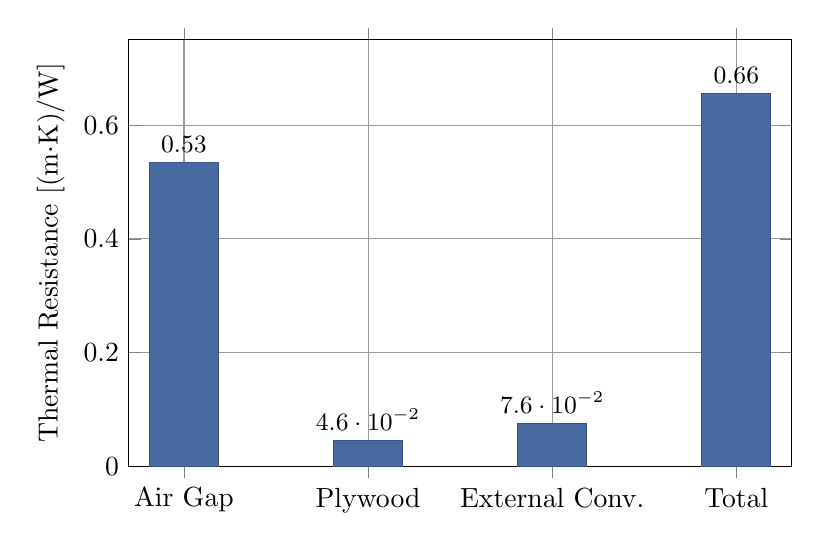
\begin{tikzpicture}
\begin{axis}[
    ybar,
    width=10cm,
    height=7cm,
    ylabel={Thermal Resistance [(m$\cdot$K)/W]},
    symbolic x coords={Air Gap, Plywood, External Conv., Total},
    xtick=data,
    ymin=0, ymax=0.75,
    bar width=25pt,
    nodes near coords,
    nodes near coords align={vertical},
    every node near coord/.append style={font=\small\bfseries},
    grid=both,
    grid style={line width=0.2pt, draw=black90!30},
    major grid style={line width=0.4pt, draw=black90!50},
]
\addplot[fill=atlantic, draw=atlantic!80!black] coordinates {
    (Air Gap, 0.534)
    (Plywood, 0.046)
    (External Conv., 0.076)
    (Total, 0.656)
};
\end{axis}
\end{tikzpicture}
\caption{Breakdown of thermal resistances. The enclosed air gap dominates.}
\label{fig:resistance_bar}
\end{figure}

\section{Summary}

\begin{table}[h]
\centering
\caption{Heat transfer summary}
\begin{tabular}{lc}
\toprule
\textbf{Parameter} & \textbf{Value} \\
\midrule
Heat loss per unit length & $106.7\unit{W/m}$ \\
\textbf{Heat loss for 30 cm} & $\mathbf{32.0\unit{W}}$ \\
\midrule
Dominant resistance & Air gap (81.4\%) \\
Plywood resistance & 7.0\% \\
External convection & 11.6\% \\
\midrule
Inner plywood temperature & 33\degC \\
Outer plywood temperature & 28\degC \\
\bottomrule
\end{tabular}
\end{table}

\section{Key Observations}

\begin{enumerate}
    \item The \textbf{enclosed air gap provides 81\% of the total thermal resistance}, making the plywood box an effective insulator despite plywood's relatively high thermal conductivity.

    \item The stagnant air acts as insulation, but natural convection (Nu $\approx$ 7) still enhances heat transfer by a factor of 7 compared to pure conduction.

    \item The plywood contributes only 7\% of the resistance---its primary function is containing the air, not insulating.

    \item To reduce heat loss further:
    \begin{itemize}
        \item Increase air gap (but this increases box size and convection effects)
        \item Add radiation shields or reflective surfaces
        \item Use insulating material instead of air
        \item Reduce cylinder temperature
    \end{itemize}
\end{enumerate}

\end{document}
